\chapter{Design and Implementation}
\label{chap:design}

Our design is inspired from the maildir format~\cite{bernstein1995using}. The maildir format stores each message in a separate file with a unique name. The mail user agent (MUA) does not have to worry about partially delivered mail: each message is safely written to disk in the \textit{tmp} subdirectory before it is moved to \textit{new}. When a mail user agent process finds message in the \textit{new} subdirectory, it moves them to \textit{cur}.

Similar to maildir, we also store all large objects in separate files. All the large objects of a database are stored under a single directory which we also call a ``BlobStore''.
The BlobStore contains three subdirectories: \textit{tmp}, \textit{curr} and \textit{old}. We will discuss purpose of these directories later in this chapter.

\section{Initializing the BlobStore}
Before starting to create blobs inside a directory, we ensure that the \textit{tmp} and \textit{curr} subdirectories have already been created. We provide a method \texttt{initBlobStore} which takes the path of a directory which is to be used as BlobStore as argument and does the initialization for us.
BlobStore is defined as a newtype. We don't expose the constructor for BlobStore, so the only way to get a BlobStore is by using the \texttt{initBlobStore} method.

\begin{program}
  \caption{Definition of BlobStore}
  \label{prog:defblobstore}
  \inputminted{haskell}{hs/blobstore.hs}
\end{program}

\section{Creating a Blob}
We provide a method called \texttt{createBlob} for creating a new blob. It takes a BlobStore as a parameter and returns a WriteContext.

\begin{program}
  \caption{Definition of WriteContext}
  \label{prog:defwritecontext}
  \inputminted{haskell}{hs/writecontext.hs}
\end{program}

WriteContext contains the file handle of just created blob, a TempLocation and a hashCtx. TempLocation stores the base directory and the filename of just created blob. The hashCtx is used to store the SHA-512 hash of the contents that has been written to the blob.

All the new blobs are created in the \textit{tmp} folder. We use Version 4 UUID~\cite{leach2005universally} to give unique names to the newly created blobs.

\section{Writing to a Blob}
We only allow to add new data at the end of a given blob. We provide \texttt{writePartial} method for this. \texttt{writePartial} takes a blob and a WriteContext as arguments and appends the given blob to the WriteContext's blob.
Once all the data has been written to the blob, \texttt{finalizeWrite} is called. \texttt{finalizeWrite} takes a WriteContext as argument and moves the blob from \textit{tmp} folder to \textit{curr} folder. We also rename the file to SHA-512 hash of its contents.
\texttt{finalizeWrite} returns a BlobId. This BlobId contains the location of the blob.
No more updates to the blob are possible after calling \texttt{finalizeWrite}.

\begin{program}
  \caption{Definition of BlobId}
  \label{prog:defblobid}
  \inputminted{haskell}{hs/blobid.hs}
\end{program}

\begin{figure}[hbt]
  \caption{Directory structure of a BlobStore}
  \label{fig:blobstore-dirstructure}
  \dirtree{%
    .1 blobstore.
    .2 tmp.
    .3 f66affb7-ad10-4583-8986-c4a6892d0120.
    .2 curr.
    .3 sha512-a75ebf9a0f109288d3eae1ecbfd89....
  }
\end{figure}

\section{Reading from Blob}
Reading is also sequential. First the \texttt{initRead} method is called which takes a BlobId as argument and returns a ReadContext. ReadContext also contains the file handle of the blob which is opened in read mode.

\begin{program}
  \caption{Definition of ReadContext}
  \label{fig:defreadcontext}
  \inputminted{haskell}{hs/readcontext.hs}
\end{program}

\texttt{readPartial} takes a ReadContext and number of bytes as input and returns those number of bytes from the blob.
While reading from a blob, you can skip ahead using the method \texttt{skipBytes}. \texttt{skipBytes} takes a ReadContext and number of bytes, \textit{b} as input and skips \textit{b} bytes ahead in the ReadContext.

\begin{table}[hbt]
\caption{Interface for operations on blob}
\label{tab:interface-blob}
\begin{center}
  \begin{tabularx}{0.91\textwidth}{lX}
    \hline\noalign{\smallskip}
    Methods & Purpose \\
    \noalign{\smallskip}
    \hline
    \noalign{\smallskip}
    \texttt{initBlobStore} & Initializes given directory to be used as a BlobStore \\
    \texttt{createBlob} & Creates a blob in the given BlobStore\\
    \texttt{writePartial} & Takes a blob and appends it to the end of the blob given in the argument\\
    \texttt{finalizeWrite} & Takes a WriteContext as input and returns a BlobId \\
    \texttt{initRead} & Takes a BlobId as input and returns a ReadContext \\
    \texttt{readPartial} & Reads a given number of bytes from a Blob \\
    \texttt{skipBytes} & Skips ahead a given number of bytes in a Blob \\
    \texttt{finalizeRead} & Completes the read \\
    \hline
  \end{tabularx}
\end{center}
\end{table}

\begin{figure}
  \caption{Order of operations on Blob}
  \label{fig:blob-operations-order}
  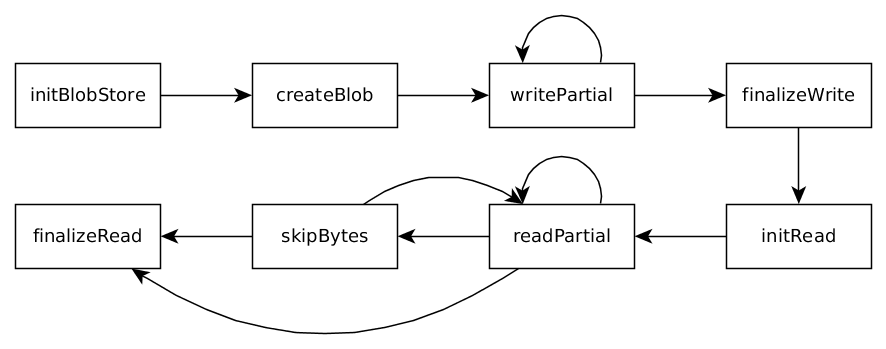
\includegraphics[scale=0.5]{figures/blob_operations_order.png}
\end{figure}

\section{Garbage Collection}
It is quite likely that the same blob would be shared by multiple ``values'' in the database. For a relational database these values are rows in a table, while for a document-oriented database, these values are documents.
Hence, we provide an interface for garbage collecting the deleted blobs.

\subsection{Starting the Garbage Collection}
The \texttt{startGC} method takes a BlobStore as argument and starts garbage collection (GC) for that BlobStore.
\texttt{startGC} does two things: It first renames the \textit{curr} folder to \textit{old} and then creates an empty \textit{curr} folder.
Once a GC has started you can not start another GC on the same BlobStore until the first one finishes - doing so will throw an error. Also, note that creation of new blobs and reading the old blobs can happen concurrently with the GC.

\begin{figure}[hbt]
  \caption{Directory structure of a BlobStore during GC}
  \label{fig:blobstore-dirstructure-gc}
  \dirtree{%
    .1 blobstore.
    .2 tmp.
    .3 1a4c5091-1295-4c9c-b8d3-8e6123a51b41.
    .2 old.
    .3 sha512-9b71d224bd62f3785d96d46ad3ea3....
    .2 curr.
    .3 sha512-11853df40f4b2b919d3815f64792e....
  }
\end{figure}

\subsection{Marking a blob as accessible}
Once a blob is marked as not deleted using the method \texttt{markBlobAsAccessible}, we move it from the \textit{old} folder to the \textit{curr} folder. This ensures that the blob does not get deleted at the end of the GC.

\subsection{End Garbage collection}
This step involves removal of all the blobs which are not accessible. The \texttt{endGC} method takes a BlobStore as argument and delete the \textit{old} subdirectory along with its contents.

\begin{table}[hbt]
\caption{Interface for garbage collection}
\label{tab:interface-gc}
\begin{center}
  \begin{tabularx}{0.91\textwidth}{lX}
    \hline\noalign{\smallskip}
    Methods & Purpose \\
    \noalign{\smallskip}
    \hline
    \noalign{\smallskip}
    \texttt{startGC} & Starts garbage collection for the given BlobStore\\
    \texttt{markBlobAsAccessible} & Marks the given blob as accessible\\
    \texttt{endGC} & Ends the garbage collection by removing all the unaccessible blobs\\
    \hline
  \end{tabularx}
\end{center}
\end{table}

\section{Concurrency}
In this section we will describe how the design described above allows concurrent access on blobs across processes.
